\documentclass[utf8]{ctexart}

\usepackage[a4paper,left=1.25in,right=1.25in,top=1in,bottom=1in]{geometry}
\usepackage{listings}
\usepackage{graphicx}
\usepackage{caption}
\usepackage{subfigure}
\usepackage{booktabs}
\usepackage{amsmath}
\usepackage{amsthm}
\usepackage{amsfonts}
\usepackage{float}
\usepackage{indentfirst}
\usepackage{tikz}
\usetikzlibrary{shapes,arrows}
\usetikzlibrary{shapes.geometric, arrows}
\usepackage{algorithm}
\usepackage{algorithmic}
\usepackage{newclude}
\usepackage[perpage]{footmisc}

\graphicspath{ {images/} }
\raggedbottom	% 令页面在垂直方向向顶部对齐
\renewcommand\qedsymbol{QED}
\newcommand{\sign}[1]{\mathrm{sgn}(#1)}
\everymath{\displaystyle}   % 行内公式采用行间公式格式排列
\pagestyle{plain}

\title{《计算机辅助几何设计》第九次作业}
\author{姓名:殷文良\qquad 学号:12435063}
\date{\today}

\begin{document}
\maketitle
\ctexset { section = { format={\Large \bfseries } } }

\section*{思考题 1}
\subsection*{1.}

    \begin{algorithm}[H]
        \caption{双$n$次Bezier曲面的de Casteljau算法}
        \label{alg1}
        \renewcommand{\algorithmicrequire}{\textbf{Input:}}
        \renewcommand{\algorithmicensure}{\textbf{Output:}}
        \begin{algorithmic}[1]
            \REQUIRE $P,n,\quad u,v\in[0,1]$
            \ENSURE $S = \sum_{j=0}^mB_{j,m}(v)\left ( \sum_{i=0}^nB_{i,n}(u)P_{i,j}\right )$

            \FOR{$j=0:n$}
            \STATE $Q[j] = \text{deCasteljau}(P[j][], n, u);$
            \ENDFOR

            \STATE $S=\text{deCasteljau}(Q, n, v);$
            \RETURN S;
        \end{algorithmic}
    \end{algorithm}

\begin{itemize}
    \item \bf{de Casteljau算法}\\
    一共要执行的线性插值次数为
    $$
    \frac{n(n+1)(n+1)}{2} + \frac{n(n+1)}{2}.
    $$
    对于3维控制顶点,每次插值需要执行$(2+1)*3=9$次浮点运算(包括加法和乘法),因此时间复杂度为
    $$
    \frac{9n(n+1)(n+2)}{2} = O(n^3).
    $$
    \begin{figure}[H]
        \centering
        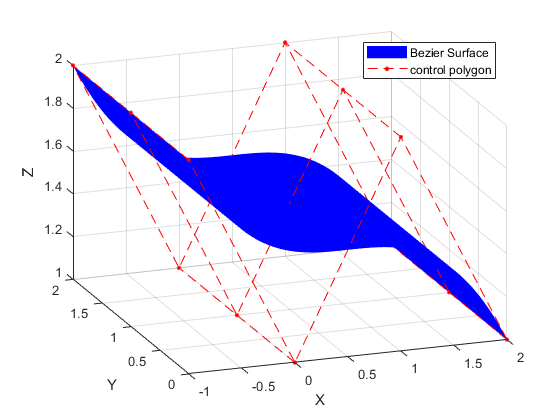
\includegraphics[width=0.8\textwidth]{bezierSurf_deCas.png}
        \caption{$2\times 3$次Bezier曲面:de Casteljau算法}
        \label{fig: bezierSurf_deCas}
    \end{figure}
    \item \bf{控制曲线算法}\\
    根据Bernstein基函数递推关系式,计算某参数处所有$n$次基函数需要执行的浮点运算次数(包括加法和乘法)为
    $$
    n(n + 1) + \frac{n(n-1)}{2} = \frac{n(3n+1)}{2}.
    $$
    对于3维控制顶点,计算$n+1$条控制曲线需要执行的运算次数为
    $$
    3 * (2n+1) * (n+1).
    $$
    最后计算$(u,v)$处的点还需执行$\frac{n(3n+1)}{2} + 3 * (2n+1)$次运算。因此,时间复杂度为
    $$
    \frac{n(3n+1)}{2} * 2 + 3 * (2n+1) * (n+2) = O(n^2).
    $$
    \begin{figure}[H]
        \centering
        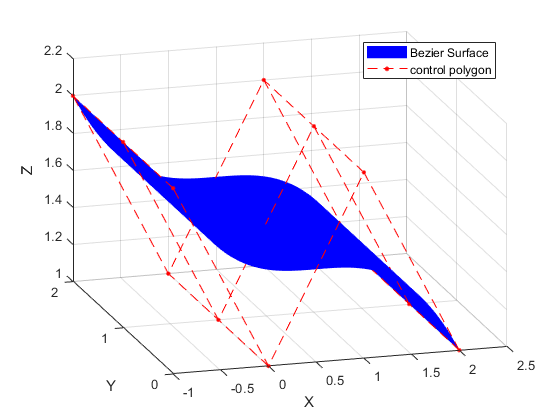
\includegraphics[width=0.8\textwidth]{bezierSurf_bern.png}
        \caption{$2\times 3$次Bezier曲面:控制曲线算法}
        \label{fig: bezierSurf_bern}
    \end{figure}
\end{itemize}

\subsection*{2.}
\begin{proof}
    由双线性曲面性质可知,
    $$
    X(u, v) = u(P_{10}-P_{00}) + v(P_{01} - P_{00}) + P_{00}.
    $$
    再由恒等式$\sum_{i=0}^niB_{i,n}(t)=nt$以及Bernstein基函数的权性可得,
    $$
    \begin{aligned}
        \sum_{i=0}^m\sum_{j=0}^nP_{ij}B_{i,m}(u)B_{j,n}(v) &= \sum_{i=0}^m\sum_{j=0}^nX(\frac{i}{m}, \frac{j}{n})B_{i,m}(u)B_{j,n}(v)\\
        &= \sum_{i=0}^m\sum_{j=0}^n\left (  \frac{i}{m}(P_{10}-P_{00}) + \frac{j}{n}(P_{01} - P_{00}) + P_{00}\right )B_{i,m}(u)B_{j,n}(v)\\
        &= \sum_{j=0}^n u(P_{10}-P_{00})B_{j,n}(v) + \sum_{i=0}^m v(P_{01}-P_{00})B_{i,m}(u) + \sum_{i=0}^m\sum_{j=0}^nP_{00}B_{i,m}(u)B_{j,n}(v)\\
        &= u(P_{10}-P_{00}) + v(P_{01} - P_{00}) + P_{00} = X(u,v).
    \end{aligned} 
    $$
\end{proof}

\subsection*{3.}
\begin{proof}
    椭球$\frac{x^2}{a^2}+\frac{y^2}{b^2}+\frac{z^2}{c^2}=1$的极坐标参数化为
    $$
    \begin{cases}
        x &= a\sin{\theta}\cos{\phi}\\
        y &= b\sin{\theta}\sin{\phi}\\
        z &= c\cos{\theta}
    \end{cases},\quad
    \theta \in [0, \pi], \phi \in [0,2\pi).
    $$
    引入两个新的参数$u,v$,定义如下:
    $$
    \begin{cases}
        u &= \tan{\frac{\theta}{2}},\quad u \in [0,\infty)\\
        v &= \tan{\frac{\phi}{2}}, \quad v \in (-\infty, \infty).
    \end{cases}
    $$
    于是得到椭球的有理参数化:
    $$
    \begin{cases}
        x &= \frac{2au(1-v^2)}{(1+u^2)(1+v^2)}\\
        y &= \frac{4buv}{(1+u^2)(1+v^2)}\\
        z &= \frac{c(1-u^2)}{1+u^2}
    \end{cases},
    \quad u \in [0,\infty), v \in (-\infty, \infty).
    $$
\end{proof}
\begin{figure}[H]
    \centering
    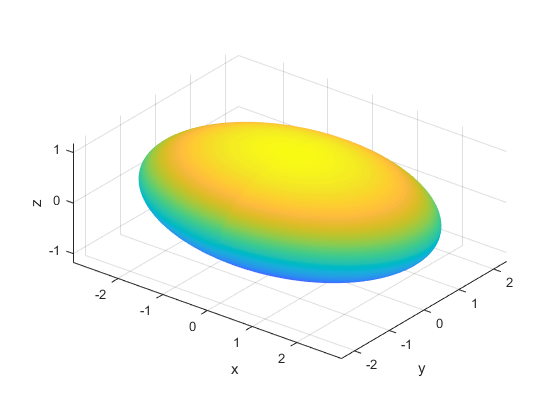
\includegraphics[width=0.8\textwidth]{ellipsoid.png}
    \caption{$\frac{x^2}{9}+\frac{y^2}{4}+\frac{z^2}{1}=1$}
    \label{fig: ellipsoid}
\end{figure}

\section*{思考题 2.}
\subsection*{1.}
\begin{proof}
设$xz$平面内有一个半径为$r$,圆心距$x,z$轴分别为$d,R$的整圆,表示为
$$
c(v) = \frac{\sum_{j=0}^6N_{j,3}(v)w_jP_j}{\sum_{j=0}^6N_{j,3}(v)w_j},
$$
其中,节点向量为
$$
V =  \{0, 0, 0, \frac{1}{4}, \frac{1}{2}, \frac{1}{2}, \frac{3}{4}, 1, 1, 1\},
$$
控制顶点和权重分别为
$$
\begin{aligned}
    \{P_{j}\} &= \{(R+r, 0, d), (R+r, 0, d + r), (R - r, 0, d + r), (R-r, 0, d), \\
    &\qquad (R - r, 0, d - r), (R + r, 0, d - r), (R+r, 0, d)\},\\
    \{w_j\} &= \{1, \frac{1}{2}, \frac{1}{2}, 1, \frac{1}{2}, \frac{1}{2}, 1\}.
\end{aligned}
$$
将$c(v)$绕$z$轴旋转得到环面
$$
S(u, v) = \frac{\sum_{i=0}^6\sum_{j=0}^6N_{i,3}(u)N_{j,3}(v)w_{i,j}P_{ij}}{\sum_{i=0}^6\sum_{j=0}^6N_{i,3}(u)N_{j,3}(v)w_{i,j}},
$$
其中,$P_{i,j}$是由$P_{0, j} = P_j$旋转生成圆得到的控制顶点;节点向量
$U,V = \{0, 0, 0, \frac{1}{4}, \frac{1}{2}, \frac{1}{2}, \frac{3}{4}, 1, 1, 1\}$;
而曲面权因子由如下公式计算
$$
w_{ij} =
\begin{cases}
    w_{0, j},\quad &j = 0, 3, 6,\\
    \frac{1}{2}w_{0,j}, \quad & j = 1,2,4,5
\end{cases},\quad
w_{0,j} = w_j, \quad j = 0,1,\dots,6.
$$

\end{proof}

\subsection*{2.}
\begin{figure}[H]
    \centering
    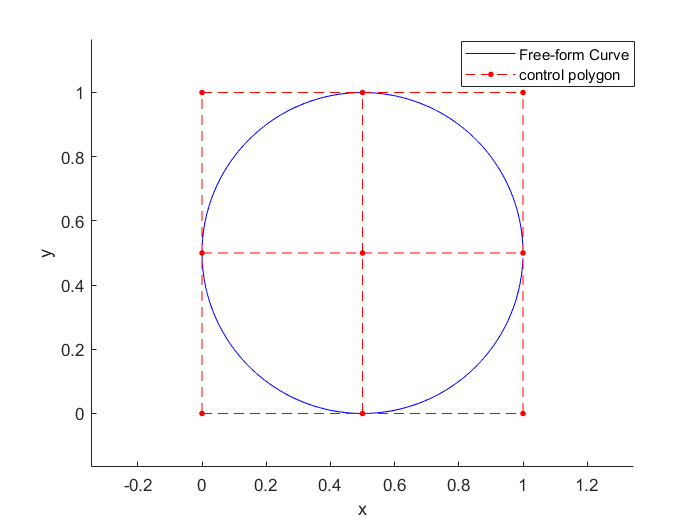
\includegraphics[width=0.8\textwidth]{ffd_1.png}
    \caption{Bézier 表示具有线性精度}
    \label{fig: ffd_1}
\end{figure}

\begin{figure}[H]
    \centering
    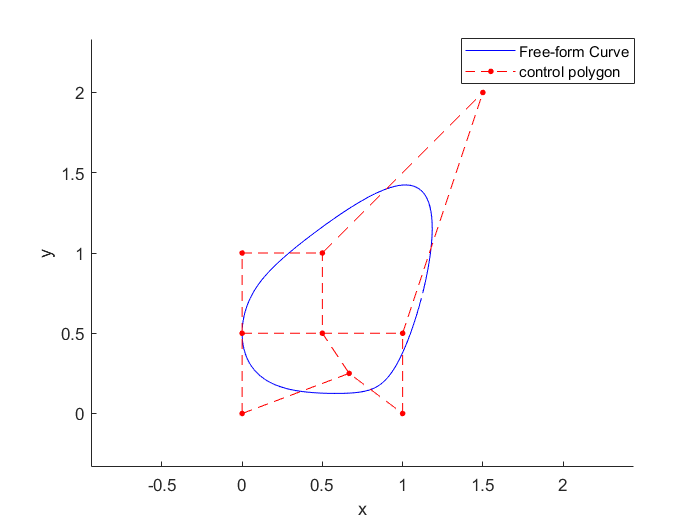
\includegraphics[width=0.8\textwidth]{ffd_2.png}
    \caption{变形后:$(\frac{1}{2}, 0)\to (\frac{2}{3}, \frac{1}{4}), \quad (1, 1)\to (1.5, 2)$}
    \label{fig: ffd_2}
\end{figure}

\subsection*{3.}
\begin{itemize}
    \item \textbf{Bezier曲面插值}\\
    \begin{figure}[H]
        \centering
        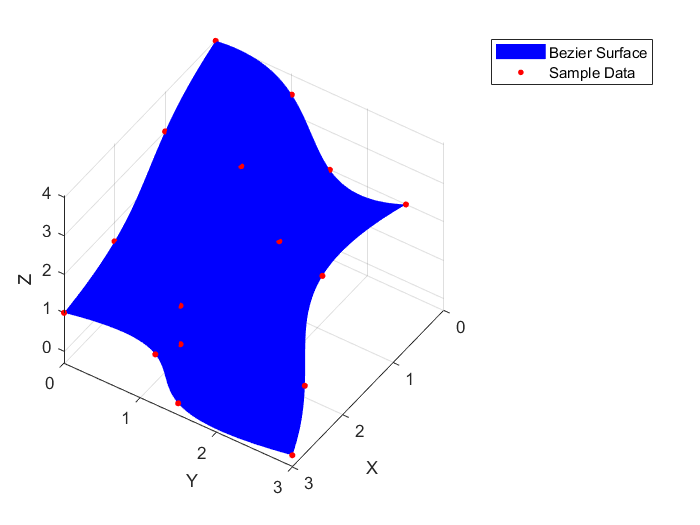
\includegraphics[width=0.8\textwidth]{bezierSurfInterp.png}
        \caption{双三次Bezier曲面}
        \label{fig: bezierSurfInterp}
    \end{figure}
    \begin{figure}[H]
        \centering
        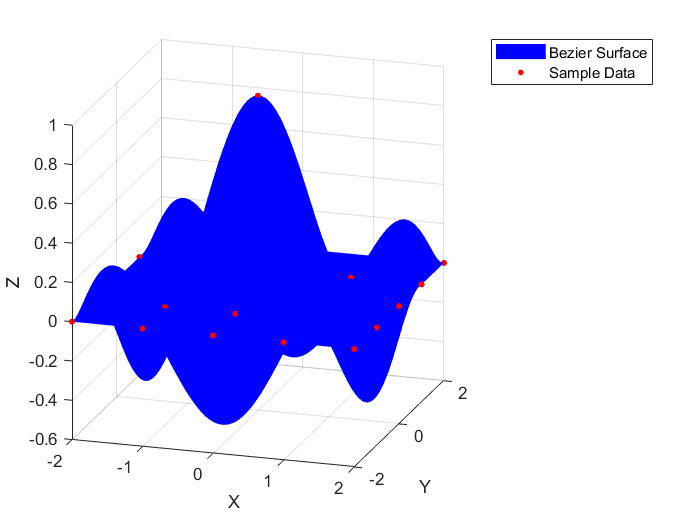
\includegraphics[width=0.8\textwidth]{bezierSurfInterp2.png}
        \caption{全局插值不能很好地处理局部数据点共面的情况}
        \label{fig: bezierSurfInterp2}
    \end{figure}
    \item \textbf{B样条曲面插值}\\
    \begin{figure}[H]
        \centering
        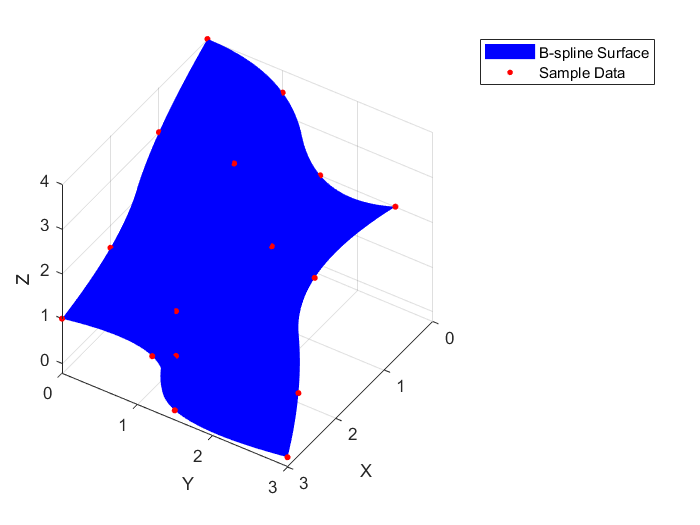
\includegraphics[width=0.8\textwidth]{bsplineSurfInterp.png}
        \caption{双二次B-spline曲面}
        \label{fig: bsplineSurfInterp}
    \end{figure}
    \begin{figure}[H]
        \centering
        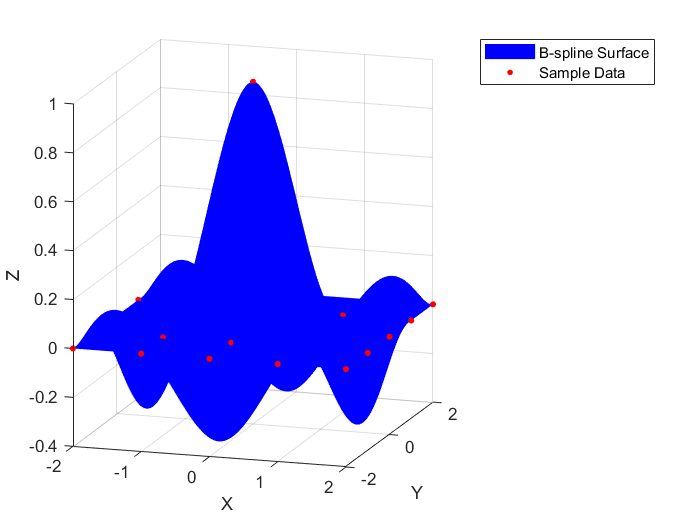
\includegraphics[width=0.8\textwidth]{bsplineSurfInterp2.png}
        \caption{双三次B-spline曲面, 全局插值不能很好地处理局部数据点共面的情况}
        \label{fig: bsplineSurfInterp2}
    \end{figure}
\end{itemize}

\end{document}
